Okay here we go.

After building up intuition on the biological features of an embryo and a model capable of (very crudely) mimicing it, we can now begin probing our model for interesting phenomena.\\
\todo{Give me all the questions again}\\
We know nature has a handful symmetry breaks which are kept enacted through self-[interacting] feedback loops. Having added a minimal number of these, we would like to see whether vivo-like gastrulation can emerge. Focusing not just the final structures; but also the individual events leading up to it.\todo{Flet\textit{ No explicit timing (BC, IC)} ind}\\
 
Once we have assessed the phenomenological validity of our solution, we can look onwards for interesting YY to study. Given our full embryo model from [individual constituents], simulating separate events, we will be looking into the interplay between these [constituents] and events. \reph\\


On the structure: In the following sections we will go through the similarities between simulation and reality, starting from simple visual comparisons, ending in detailed quantifications. We will do these for the different events (A1-A4) and embryo domains. Afterwards, we will be looking at removing different active parts of the simulated embryo, comparing the results to known real-life mutants. This will finally lead us to an analysis of the YYY-interactions, including parameter sensitivity and YYY. 

Qualitative Agreement
Quantitative Agreement
Mutants vs In Vivo
Mutant vs in Silico
"New mutants"
Stability Analysis



\newpage

\section{Qualitative Agreement}
While the Drosophila embryo has been studied for decades, it is only relatively recently computer vision has gotten to a point where quantitative analyses of the more than 5000 cells has turned feasible. Therefore, like most of the fields history, we will start with examining the visual agreement between the morphology of simulation and data.\\

For all Figures in this paper. If nothing else is noted, the run is [define run]. As the time of invagination of the YYY (stage YY in the overview) is about 12 minutes, the timing of the simulation is defined likewise allowing for comparisons in "minutes".

% To remind ourselves of our goals, we will quickly summarize Figure .

It is easy to hide behind numbers and YYY analyses, so to combat this, we will go through the individual main morphological events (A1-A4 from Figure \ref{fig:big-timeline})\todo{REMEMBER TO CORRECT NUMBERS}. WE can then compare to imaged embryos to make certain we have the phenomenological agreement.

On the following page, our best in silico model and corresponding frames from a video by [Stas' group] can be seen and compared:

\newpage

\begin{figure}[H]
    \centering
    \vspace*{-1cm}\hspace*{-1cm}\makebox[\textwidth]{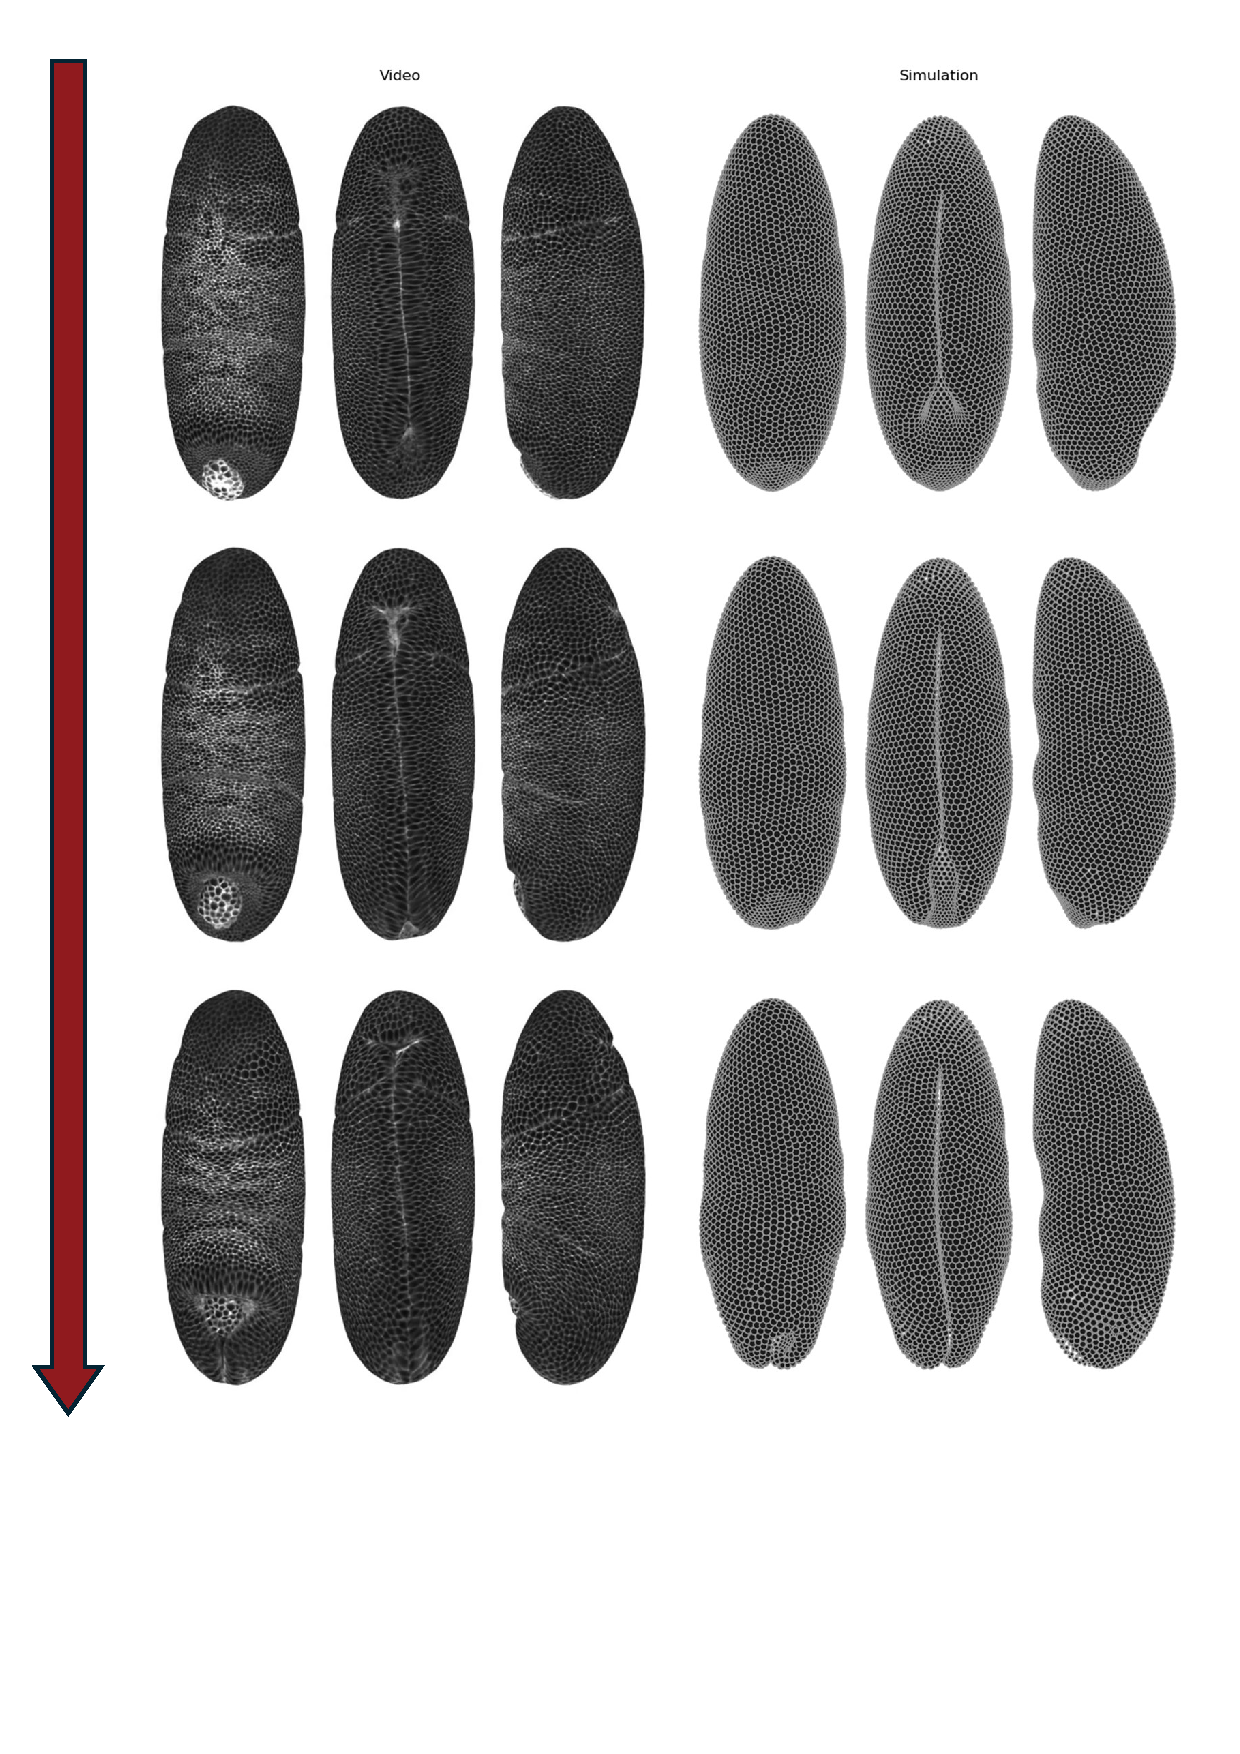
\includegraphics[width=0.85\paperwidth]{chapters/Results/figures/compare_to_vid_timeline.pdf}}
    \caption{Caption on next page}
    \label{fig:big-visual-comparison}
\end{figure}
\newpage
\addtocounter{figure}{-1}
\begin{figure} [t!]
  \caption{(Previous page.) \\A full page visual comparison between three timesteps of the simulation and in vivo imaging. 
  Each row consists of a single time-step. \\\textbf{Left:} In vivo. \textbf{Right:} In silico.\\Within each row, the embryo is show from the top (dorsally), bottom (ventrally) and side (laterally), with the back end (posterior) pointing downwards.
  }
\end{figure}

Comparing, we can see that from a naïve inspection, not only has the general shape, timing and YYY been recapitulated, but YYY.  Given the relatively simple model and few specific alterations, this already seems notable \note{maybe be more humble}, but to completely understand the agreements between data and simulation we will need to scrutinize the individual pieces using some visual aids. We will now go through different parts of the embryo, comparing them to in-vivo imaging when available.


\subsection{Ventral Furrow (\vf{A1})}
The the first sign of movement on the embryo is on the belly where a distinct cleft begins forming. \\
This is called the \vf{ventral furrow} and is the first point of creation for the tubes that will become the gastrointestinal tract.
As the furrow closes, the internalized cells form a tube with a recognizable light bulb-shape in the cross section. 

Below, in Figure \ref{fig:VFComparison}, a comparison between a cross section of our simulation and in vivo imaging can be seen.

\begin{figure}[H]
    \centering
    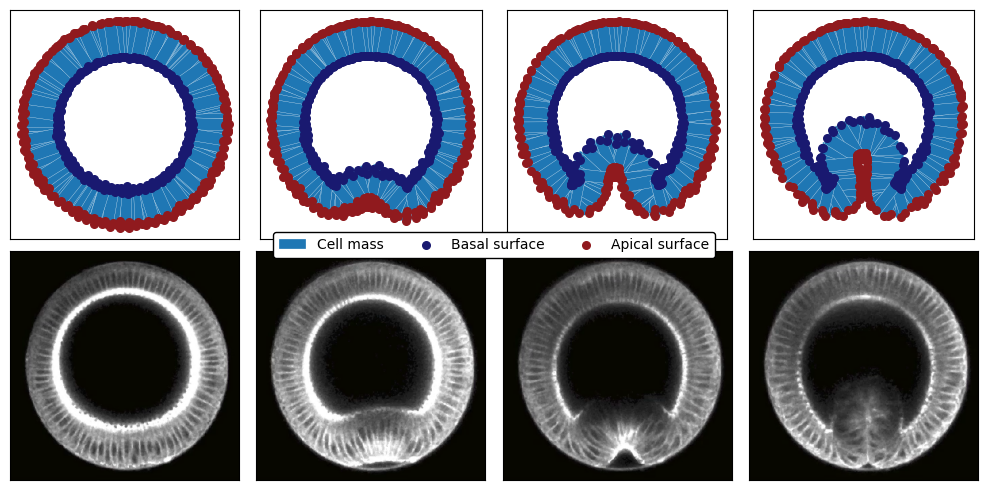
\includegraphics[width=1\linewidth]{chapters/Results/figures/VF_comparison.png}
    \caption{A comparison of simulation and frames from video of live growth. \\\textbf{Upper row}: Simulation. \textbf{Lower row}: Multi-photon microscopy. \\For ease of visualisation, each cell in the simulation is displayed as a rectangle with the longer side aligning with each cells AB-axis. Each frame is taken at equally spaced time intervals (Cross section video from \citeAY{conte2012biomechanical})}
    \label{fig:VFComparison}
\end{figure}

In our simulation, the invaginating tissue extends slightly more towards the center.\footnote{But this also seems to be a problem for the state of the art \citeAY{allena2010simulation} who did full vertex-based simulation of \textit{only} the ventral furrow}  This is especially noticeable closer to the anterior tip.
But in general, we find the formation of the ventral furrow to have been reasonably accurately recreated both during development and when fully formed. 


\subsection{Germ-band}
The largest cell group on the blastoderm is the Germ-band which fills most of the lateral sides. As mentioned in Section \ref{sec:drosophila-embryo-detail}, it is generally agreed that the Germ-band is one of the main drivers of anterior-posterior motion (although it remains disputed how).

In Figure \ref{fig:germbandCompare} a text-book diagram of the motion of the germ-band can be compared with the shape of the germ-band in the first and last frame of our simulation. 
\begin{figure}[H]
    \centering
    \begin{subfigure}[b]{0.3\textwidth}
        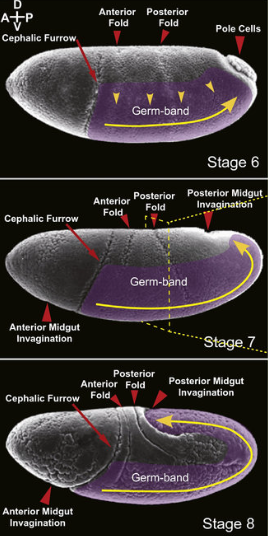
\includegraphics[width=\textwidth]{chapters/Results/figures/compareGB.png}
    \caption{Figure taken from \citeAY{kong2017forces} }
    \end{subfigure}
     % \hfill
    \begin{subfigure}[b]{0.61\textwidth}
    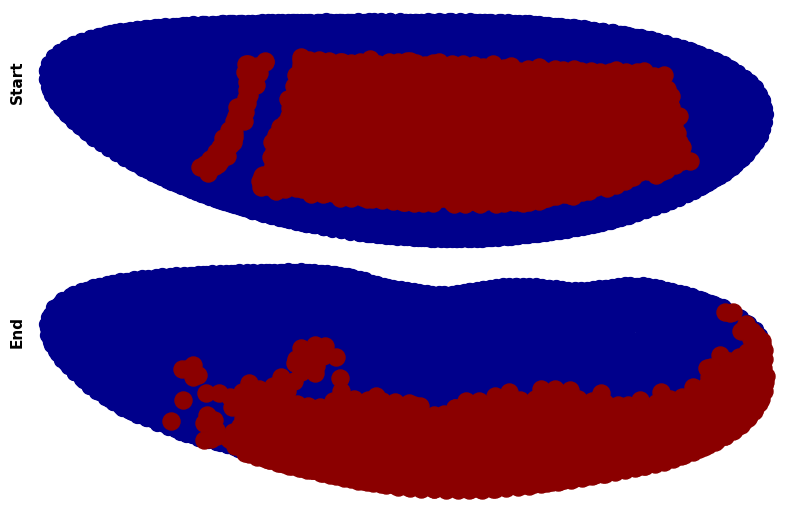
\includegraphics[width=\textwidth]{chapters/Results/figures/gb_firstframe_lastframe.png}
    \caption{Simulation with colored in Germ-band}
    \end{subfigure}
    \caption{A visual comparison between a diagram of the germ-band cells and the cells as defined in our simulation\\Note: The blue line separating the germ-band in the initial frame is a quirk of the gene-expression-cutoff as described in Section \ref{sec:drosophila-embryo-detail}.}
    \label{fig:germbandCompare}
\end{figure}


In general we see a great agreement in the morphological timeline of the germ-band between simulation and data. Both the migration ventrally and dorsal 'rise' at the posterior tip. For a representation of the motion of individual cells in the germ-band, see Figure \ref{fig:GBMovements} below:
\begin{figure}[H]
    \centering
    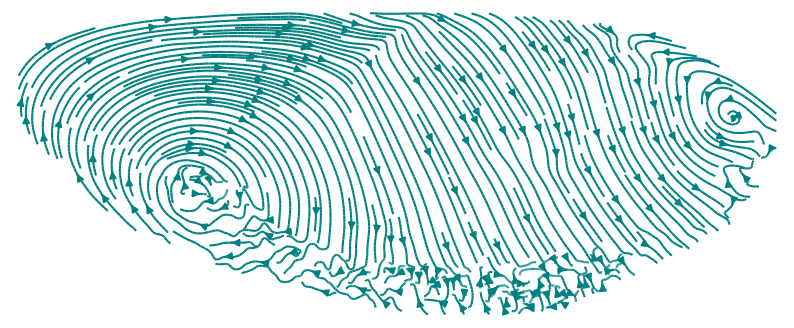
\includegraphics[width=1\linewidth]{chapters/Results/figures/streamplot2.png}
    \caption{Streamplot }
    \label{fig:enter-label}
\end{figure}

\begin{figure}[H]
    \centering
    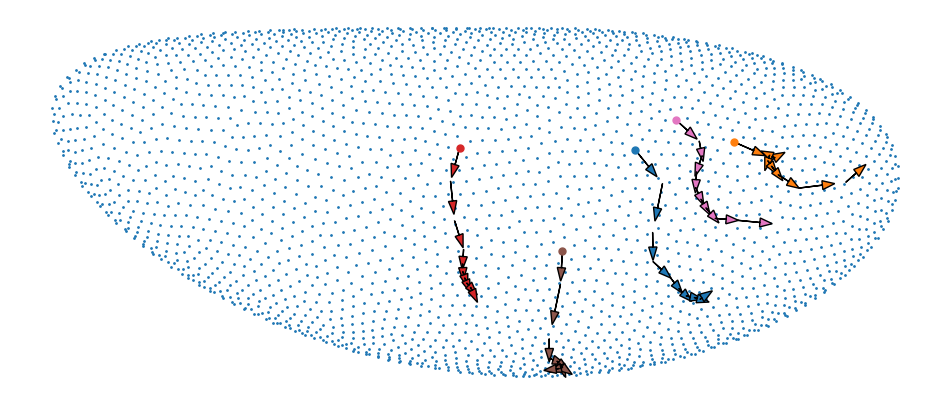
\includegraphics[width=1\linewidth]{chapters/Results/figures/movements.png}
    \caption{\todo{Remove some of the cells -- it's cluttered. Change color over time}}
    \label{fig:GBMovements}
\end{figure}




\subsection{General morphology}
In the literature, a common way of visualizing the changes in both local and global structure, consist of drawing straight lines on the embryo at the onset of gastrulation. How these lines translate and skew over time is very descriptive for how the form changes. An example in both data and simulation can be seen in Figure \ref{fig:band-movements-stas}.

\begin{figure}[H]
    \centering
    \makebox[\textwidth][c]{\hspace*{-1cm}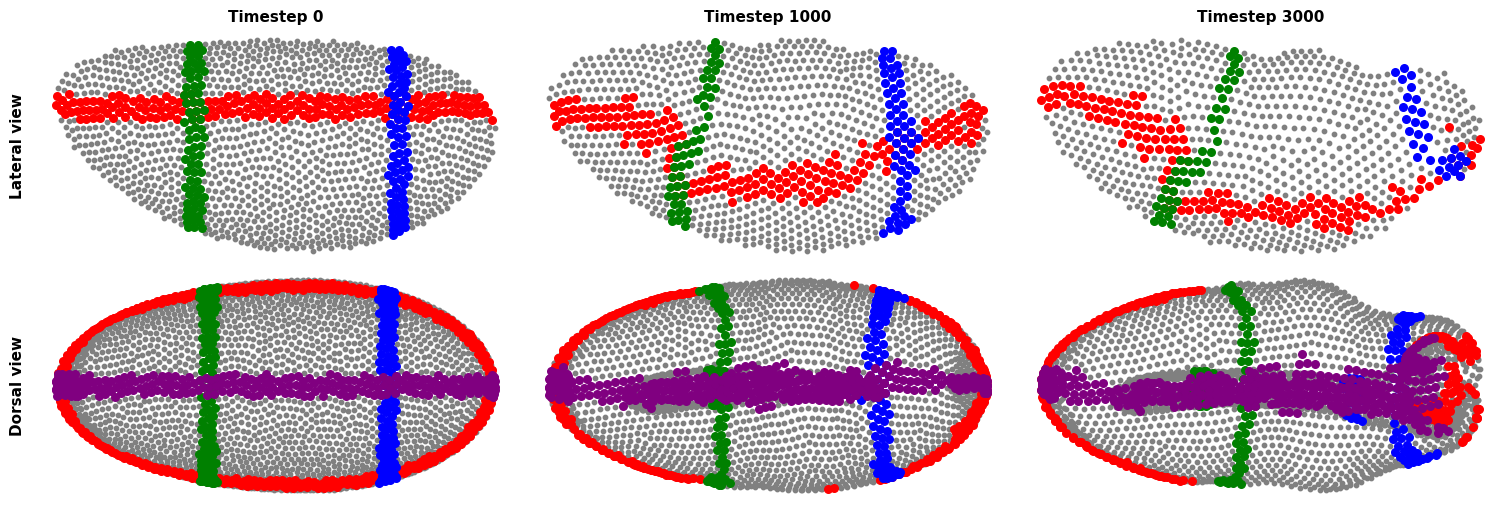
\includegraphics[width=1.\linewidth]{chapters/Results/figures/band_movements.png}}
    % \caption{My simulation. Compare to figure \ref{fig:band-movements-stas}}
    % \label{fig:band-movements}
\end{figure}
\begin{figure}[H]
    \centering
    \makebox[\textwidth][c]{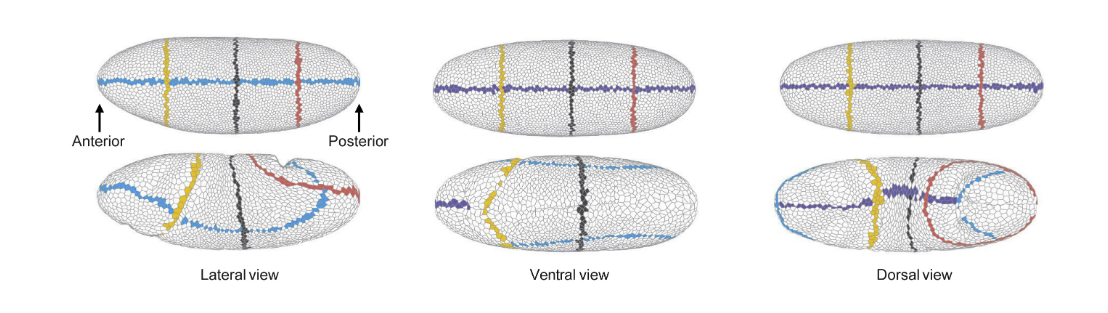
\includegraphics[width=1.\linewidth]{chapters/Results/figures/compareStasGBShape.png}}
    \caption{Positions of specific bands over time. \\ \textbf{Top row:} Simulation. Three time steps from two different angles.\\ \textbf{Bottom row:}  Segmented images (from \citeAY{stern2022deconstructing}). \\\todo{write better descr.}}
    \label{fig:band-movements-stas}
\end{figure}

This juxtaposition allows for some interesting observations:\\
As is evident, there is a general agreement between both local and large-scale changes in embryonic form. 

In our simulation, the posterior tip has some trouble after invagination and the lines becomes muddled.

Where the cephalic furrow is supposed to be (green vertical line in simulation), the epithelial sheet has less wiggle room in simulation than what is needed and also struggles to move fluidly.





% \subsection{Daniel}
% \todo{Make use of section or cut}
\section{Quantitative Agreement}

\todo{Give me all the questions again}
While visual inspection of our simulated morphogenesis is interesting, we are physicists and would like some quantification of the model performance.

It was stated earlier that quantitative data is tough to come by. But recent technical advancements in microscopy and cell-segmentation has given rise to the possibility of large-scale, automated analyses.\cite{stern2022deconstructing}

We will now go through \textit{quantitative} explorations of the agreement between our model and data collected in vivo. 


\subsection{Movements}

While the information lies in the initial conditions, it is the dynamics of the system we are interested in recreating. To explore this, we use data as collected in \citeAY{stern2022deconstructing}. 
The data-set consist of machine-tracked cell positions in 3d-space.

As we have no way of doing any one-to-one cell comparisons, the following measure was devised: 

Look at the recent motion vector of each cell. Compare these to the average motion vector of the 10 spatially closest cells in data. 
Then, find the angle between the cells motion and the average motion vector. The resulting (acute) angle difference is between 0 and $\pi$. Finally, scale this number to be between 1 and 0, giving a measure where 1 is perfect agreement.
This should hopefully give us an estimate of the agreement to the general kinematics for the different cells.

Below (in Figure  \ref{fig:motionAgreementExample}), the resulting analysis can be seen, were each motion vector is colored according to their agreement with the data.

\begin{figure}[H]
    \centering
    \makebox[\textwidth][c]{
    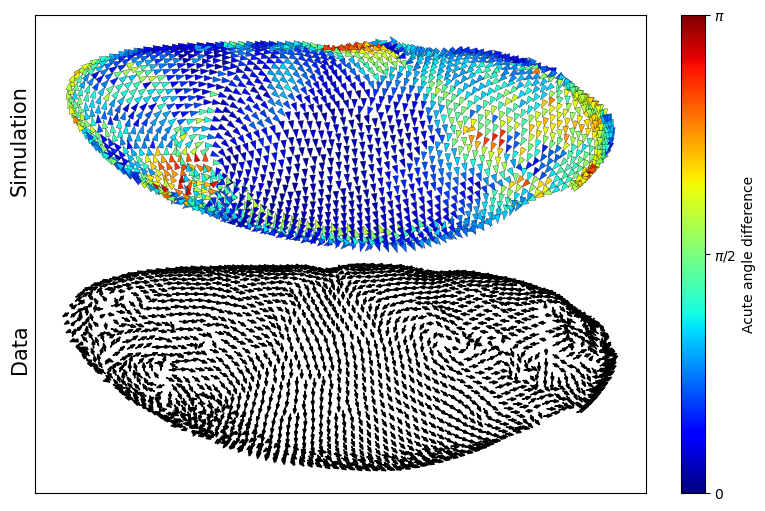
\includegraphics[width=0.9\linewidth]{chapters/Results/figures/movement_vectors_example.png}
    }
    \caption{Snapshot of motion vectors for each cell in simulation and average motion at each cells position. \todo{larger label to colorbar, write time point somewhere}}
    \label{fig:motionAgreementExample}
\end{figure}

It can be seen that at this specific time point, the agreement ranges from surprisingly good to predictably bad. Why we do not except perfect alignment will be discussed later.

Averaging this score over the whole embryo for every time point we get the following relation:

\begin{figure}[H]
    \centering
    \makebox[\textwidth][c]{
    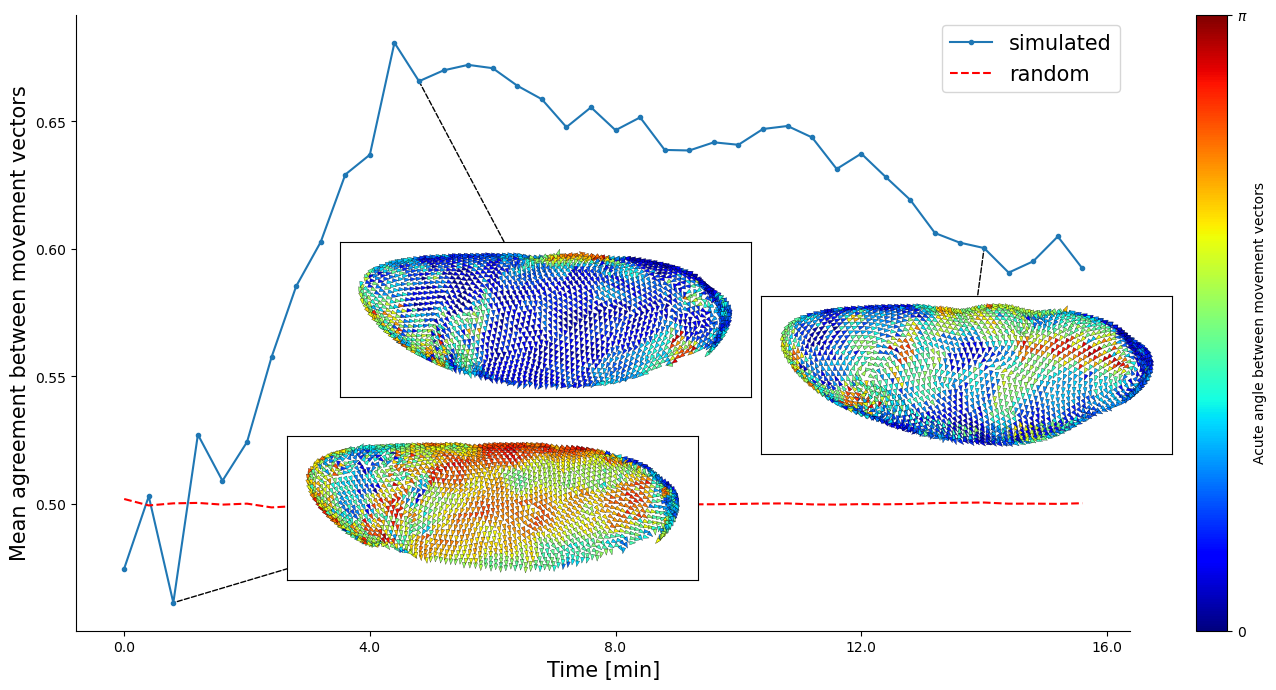
\includegraphics[width=1.3\linewidth]{chapters/Results/figures/movement_vectors_normal.png}
    }
    \caption{The average motion-vector agreement across the full embryo as a function of time\\
    The red \textit{random}-line is a simulated embryo where every direction of motion is uniformly randomly chosen. \todo{explain x-axis}}
    \label{fig:motionAgreement}
\end{figure}


In general, we see a consistent, well-above average overlap between data and simulation. 

From the previous sections, we had some intuition that our simulation visually followed the general flow of the morphogenesis. Figure \ref{fig:motionAgreement} can now   gives us some quantitative confidence that the motion of the individual cells also align with the data.

It is very clear that in the first couple of minutes our simulation and reality does not completely agree. This will be a recurring theme.

An important note: The original data only supported motion-tracking on the exterior surface of the embryo.\footnote{Another important note is: Convergent extension is by its very nature based on the global motion being being different from the motion of the individual (see Figure \ref{fig:ConvergentExtensionDiagram}). Having a per-cell agreement is almost contradictory to this type of cell motility. 
}

We will now be looking at the integrated error over the full run. Mapping the resulting "average lifetime error" back onto the initial positions we can see how the error is spatially distributed:
\begin{figure}[H]
    \centering
    \makebox[\textwidth][c]{
    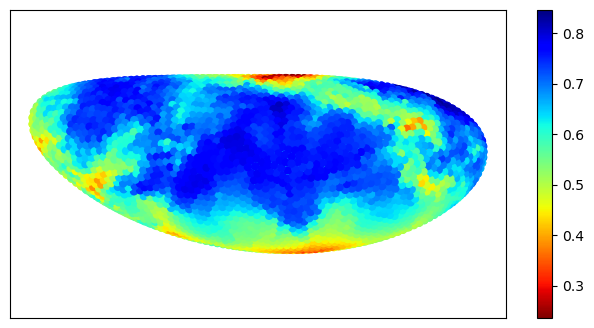
\includegraphics[width=0.8\linewidth]{chapters/Results/figures/movement_mapped_normal.png}}
    \caption{The motion-vector agreement across the full run mapped back onto their original positions \todo{colorbar label}}
    \label{fig:}
\end{figure}

The in silico motion of the germ-band seem in great agreement with data, especially given how far the individual cell travels.
Because of the way the imaging was done all invaginations (the ventral furrow for example) will automatically have low agreement.
On top (the dorsal side), the sheet usually buckles and folds, this was not part of our simulation and can also be seen to not agree with nature. \\
Even though most of the anterior (leftmost) part of the embryo has little motion until later stages, the head-tissue was pretty early deemed outside of scope of the current project.

This, along with the fact that any invaginating cells automatically will be penalized, gives us the idea of looking at the agreement for specific parts of the egg.



\begin{figure}[H]
    \centering
    \makebox[\textwidth][c]{
    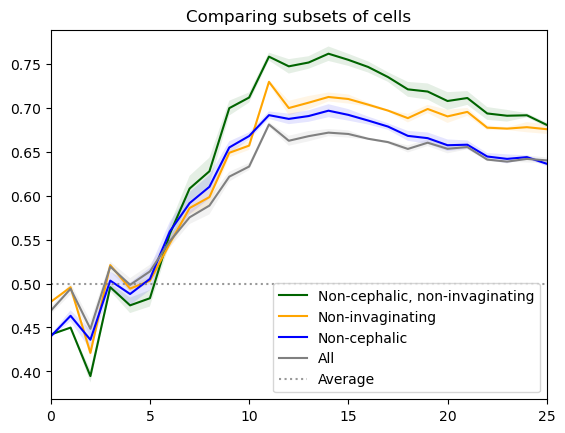
\includegraphics[width=1\linewidth]{chapters/Results/figures/movement_vectors_normal_subsets.png}
    }
    \caption{The motion-vector agreement across the full embryo as a function of time. For confidence is the stability of the current solution, all lines and shaded areas are averages and and standard deviations of three runs using identical parameters but different seeds. \todo{Fix x-axis}}
    \label{fig:vector-subsets}
\end{figure}

In Figure \ref{fig:vector-subsets}, we tried limiting the agreement analysis to only look at subsets of the embryo:

Removing cells in the Ventral and Posterior areas that were apically constricting (Non-invaginating)
Anything in the head area was discarded (Non-cephalic)

Focusing on the parts of the embryo with a good possibility of overlap with data, we get to almost 0.8 average cell-motility agreement.  

\todo{Conclude}


\subsection{Timing}
Cells have been shown to have remarkably precise internal clocks\footnote{cool footnote with a remarkable number\cite{cellinternal}} and chemical gradients in the embryo changing across timescales from seconds to hours\cite{shvartsman2008dynamics}. There is also the "biological clock"\cite{johanolsen2} that proteins themselves have dynamic structure that can change over time.\cite{johanolsen1}. But there is no evidence for any specific timing in stages 5-7 [citation needed]. We would like to stress the importance of the result that we seem to have recapitulated some of the long-term dynamics completely without any explicit time-dependent parameters. This could be seen to corroborate our thesis that  initial conditions and an inter-cellular rule set is sufficient for some of natures more complex morpologies to arise. \todo{move to conclusion /discussion}


\subsection{Strain}
As the tissue warps and skews, the cells are both subject to- and drivers of- stress and strain on the cell walls. This is one of the most widely studied parts of structural changes in morphogenesis.

While our simulation neither includes cell walls nor explicit strain calculations, a method has been developed which we can utilize. The Green-Lagrangre algorithm,\footnote{The algorithm and implementation is written out in Section \ref{App:Strain-Calculation} in the Appendix} as utilized in \citeAY{butler2009cell} among others, looks at local deformations in the tissue. In Figure \ref{fig:strain} the results of an implementation can be seen and compared to a graph on data

\begin{figure}[H]
    \centering
    \begin{subfigure}{0.45\linewidth}
        \centering
        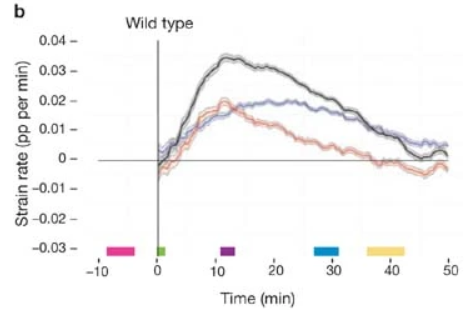
\includegraphics[width = \linewidth]{chapters/Results/figures/strain_rate_extrinsic.png}
    \end{subfigure}
        \begin{subfigure}{0.45\linewidth}
        \centering
        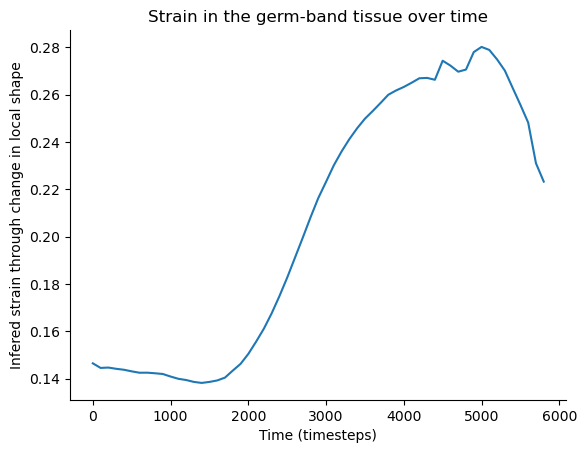
\includegraphics[width = \linewidth]{chapters/Results/figures/strain_smoothedpng.png}
    \end{subfigure}
    \caption{Comparison between Figure 1 from \citeAY{butler2009cell} (\textbf{left}) and the inferred strain in our simulation (\textbf{right}).\\
    We both see a quick rise followed by a fall-off at time of invagination of the posterior\\\todo{Explain the leftmost plot or find another that shows the same with only one line}}
    \label{fig:strain}
\end{figure}

In the first 12-15-minutes we see a rising strain, ending at the point of internalization of the germ cells ($\approx12$minutes). In our simulation, the strain has a delayed onset. The fact that the first 2 minutes have a central difference from ground truth shows up again.\\

Conclude?\\

Tie into next\\


\subsection{Ventral Furrow}
I would love to quantify the accuracy of our simulated ventral furrow.
I am guessing we can do a cell-center fit of Figure \ref{fig:VFComparison}.
Is this out of scope? Yes. Would it be cool? Also yes.
\newpage
\section{In Silico Mutants}
\todo{Give me all the questions again}
Having a complete simulated pipeline from (simplified) morphogen to (approximate) morphogenesis, opens the door for some intriguing explorations into our model and its relation to nature.\\

A large branch of developmental biology consists of discovering or creating mutated genotypes and cataloging the resulting organisms. 
Our model also allows for the creation of genetically-variant embryos by changing the response to one or more of the simulated morphogens.\\

To introduce this section we will need to shortly explain the four most prevalent "mutants" as the effects of these will be explored. 

\subsection{The mutants}
\subsubsection{No Posterior Midgut (PMG)}
The PMG is the name for the invagination that happens at the posterior to internalize the pole cells (stage 4 on Figure \ref{fig:big-timeline}).

In [cite Stas], they show that the chemical signals produced by the protein \textit{Hkb} initiates apical constriction around the posterior tip. In \textit{Hkb}-deficient mutants the lack of posterior invagination has a clear effect: The built up pressure from the extending germ-band causes the whole epethilium to twist. This has given the \textit{Hkb}-mutant the nickname "Corkscrew".\\

In Figure \ref{fig:corkscrew-comparison}, a video of the corkscrew mutant can be compared to our simulation after removing the cells ability to react to \textit{Hkb}.

 
\begin{figure}[H]
    \centering
    \makebox[\textwidth][c]{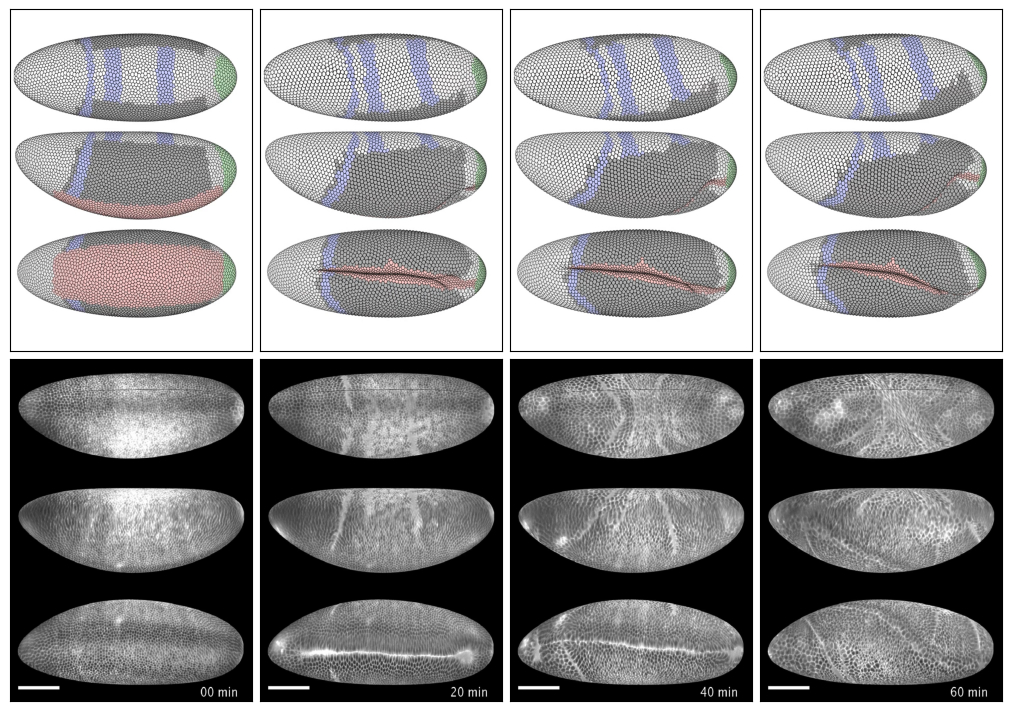
\includegraphics[width=1.2\linewidth]{chapters/Results/figures/corkscrew_comparison.png}}
    \caption{A purely visual comparison between our simulation (\textbf{top}) and the \textit{Corkscrew} phenotype (\textbf{bottom})from \citeAY{smits2023maintaining}. In both cases we see a "twisting" motion.}
    \label{fig:corkscrew-comparison}
\end{figure}
% Twist and shout

Comparing the reaction of these In Silico Mutants to real life phenotypes gives us a hint thatYYY

\subsubsection{No Ventral Furrow}
When knocking out the \textit{Twist} and \textit{Snail} genes, which, as you might remember, are primary organizers of apical constriction, the ventral furrow fails to form (stage 1 on Figure \ref{fig:big-timeline}).

The resulting embryo does not move the germ-band downwards, making the pressure exerted by this unable to move the posterior "upwards" 
% \url{https://genesdev.cshlp.org/content/5/9/1568.full.pdf}
% We are seeing the right thing
% Comparing We are seeing the right thing.
\todo{Make figure}


% \subsection{Auxiliary(cephalic furrows}

% In the absence of controlled folding of the dorsal tissue, the pressure from the extending Germ Band, can lead to other folds(?) \url{https://brunovellutini.com/posts/cephalic-furrow-thread/}

% This is key to both understanding why the invaginated posterior end does not travel further anteriorly.

% Also the large scale morphology change some runs had.

\subsubsection{No active intercolation / germ-band}
\label{sec:mutantNoGB}

When removing the patterning that is believed to be responsible for convergent extension in the germ-band, something surprising happens. It has been show (By \citeAY{butler2009cell} for example) that more the morphogenesis is driven by more than Convergent Extension, and that \textit{germ-band}-mutants are still viable. This comes from the fact that cell-shape change overtakes the movement.

In our simulation, we have no cell shape change to help alleviate the lack of motion, but as the ventral furrow still invaginates and expands we still see some movement. 
\todo{Make figure}


% We know that \textit{Runt} and \textit{Even skipped} are upstream . The litterature is conflicted, but the general theory is, that the patterning allows for a coherent orientation of the planar cell polarity. 

% PCP-orientation was set at the intial step of the simulation as pointing in the distinct direction defined by the interspersed \textit{Runt} and \textit{Even skipped} patterning.
% The results are interesting, albeit very uneventful, as
% In the litterature  \cite{butler2009cell} more the morphogenesis is driven by more than Convergent Extension, and unstriped mutants are still viable, unlike our case where nothing happens.

% Seems to be a clear indicator for active cell shape change being a vital part of... 

% TODO: Discuss level of abstraction in the model 

\subsection{Combining and comparing to each other}
Given that we have a world-first [citation needed] full embryo model, we can do some interesting in-silico experiments: A fascinating part of the morphogenesis across all ::: is the interplay between the multiple spatially separated dynamical parts of the embryo. We will in this section analyse how they interact. \todo{Rephrase}

We will be doing this analysis in two ways: Firstly by comparing the different virtual 'phenotypes' to our baseline model. Secondly by comparing to the motion data as used in previous sections. Finally we will be making an interaction-matrix, quantifying the resulting compromises and cooperation.  

\subsubsection{Pole Cell Migration}

We will now introduce the metric \textit{Pole Cell Migration} as a virtual metric for the success of the gastrulation. The Pole Cell Migration is defined as the angle change of the posterior tip in the lateral plane. That is, in degrees, how far around the embryo the posterior has moved.\todo{make figure? or just explain better} In Figure \ref{fig:PCM-mutants} a comparison of multiple runs of the known mutants described earlier can be seen and compared to the wild-type.

\begin{figure}[H]
    \centering
    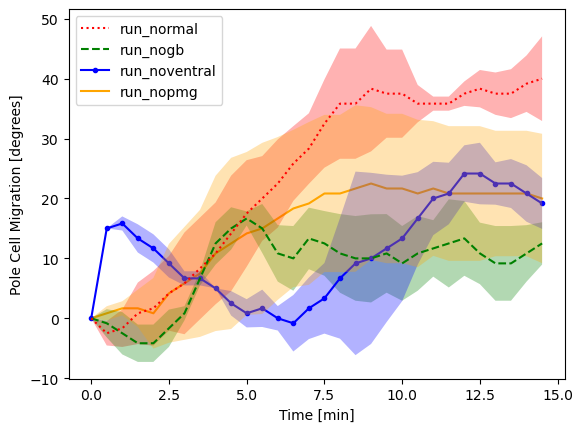
\includegraphics[width=1.\linewidth]{chapters/Results/figures/compare_PCM.png}
    \caption{\todo{Explain,}\todo{Change colors into domain-colors}}
    \label{fig:PCM-mutants}
\end{figure}


Videos of the individual runs can be found in Section \ref{App:videos} in the Appendix, but a lot of the dynamics of the system can be gathered from the motion of the posterior tip. We can see that:\\
\textbf{Normal (red):} This is the normal run. A ramping movement until reaching the point of posterior invagination at about 20 degrees. \\
\textbf{No Germ-band (green):} At first the tip moves towards the invaginating ventral furrow. As this expands slightly there is still a tendency to move the tip dorsally, but there is not enough force for the posterior tip to progress more than 5 degrees. \\
\textbf{No Ventral Furrow (blue):} Firstly, when no tissue is pulled into the ventral side, the germ-band pushes the posterior tip slightly upwards. This is negated as the pressure ultimately comes from the 'port' and 'starboard' sides, not translating the pole cells upwards.\\
\begin{wrapfigure}{l}{0.\textwidth}
    \centering
    \hspace{-3cm}
    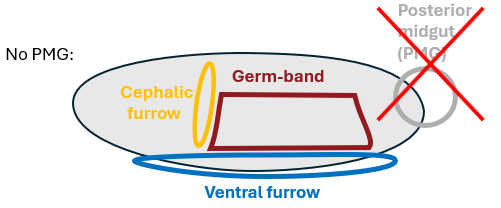
\includegraphics[width=0.5\linewidth]{chapters//Results/no_pmg_mutant_schematic.png}
\end{wrapfigure}
\textbf{No PMG (yellow line):} Here we see a possible breakdown of this metric. None of the corkscrew-twisting is captured and the lowering of PCM does not capture just how unviable an embryo with this mutation is.  


\subsection{Combining and comparing to data}
While comparing internally is interesting and can say a lot about the dynamics, we wanted a short detour where we recreate Figure \ref{fig:motionAgreement}, seeing how each mutation changes the motion-vectors. The results can be seen in Figure \ref{fig:compare-motionAgreement} below:

\begin{figure}[H]
    \centering
    \makebox[\textwidth][c]{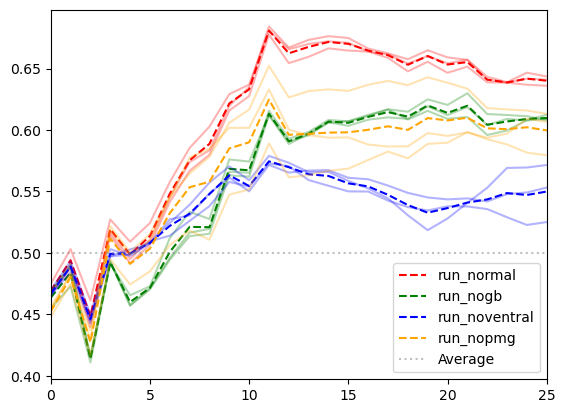
\includegraphics[width=1.3\linewidth]{chapters/Results/figures/PLACEHOLDER_compare_movement_vectors.png}}
    \caption{ Y-axis defined like Figure \ref{fig:motionAgreement}. \todo{This is an important plot. Remake in higher quality with  better legend and axis labels}}
    \label{fig:compare-motionAgreement}
\end{figure}
It is comforting to see that the motions are 
\todo{Find something interesting to discuss}

The "No Germband"-mutant is surprisingly good. We think this is due to the fact that only the angles between the motions matter: If the cell-sheet moves along the right direction, it does not matter whether they move far enough.   

But when are the different parts important? To figure this out we have the following figure:

\begin{figure}[H]
    \centering
    \makebox[\textwidth][c]{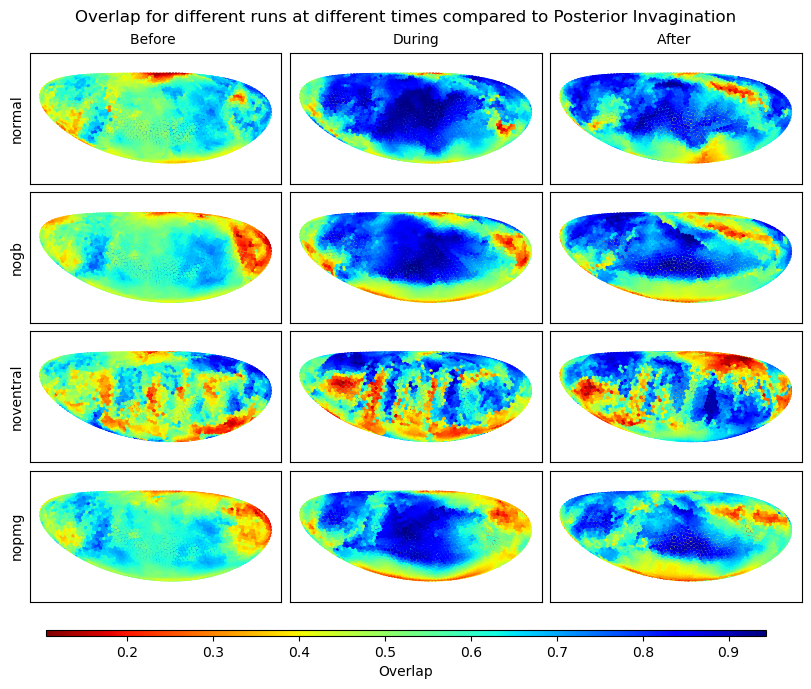
\includegraphics[width=1.3\linewidth]{chapters/Results/figures/Compare_all_movements.png}}
    % \caption{This is the main plot of the thesis. Y-axis is sum of y-axis of over all times in Figure \ref{fig:motionAgreement}}
    % \label{fig:compare-motionAgreement}
\end{figure}
\todo{I feel like there is a lot of meat on this figure. Discuss!}


\section{Interaction Matrix}
For a more granular approach, we boil the PCM down to a single number quantifying the total dorsal motion. In the matrix in Figure \ref{fig:PCM-matrix} the combined effects of missing any two can be seen (once i make it) together with the data-quantified overlaps:
% \footnote{emitting about 7kg of CO2 \url{https://mlco2.github.io/impact} }
\begin{figure}[H]
    \centering
    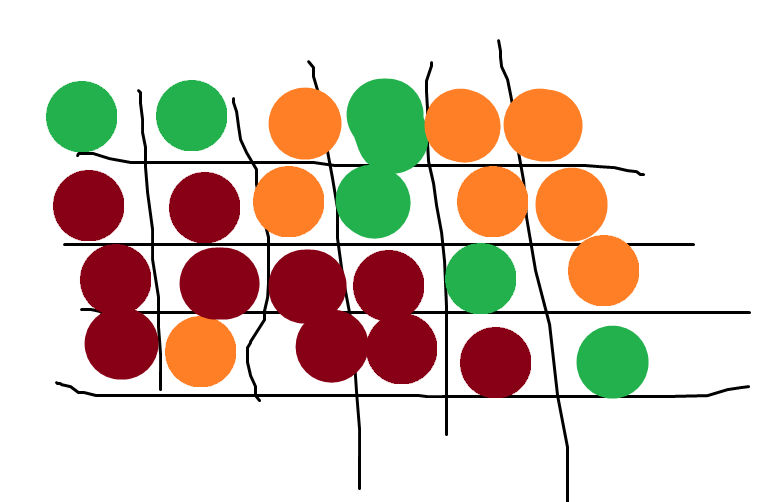
\includegraphics[width=1.\linewidth]{chapters/Results/figures/placeholder_domain_matrix.png}
    \caption{Not done yet}
    \label{fig:PCM-matrix}
\end{figure}

\todo{Find something interesting to discuss}

\section{Parameter Sensitivity Analysis}
No good examination of a model is complete without a Parameter Sensitivity Analysis. That is why I will be making one this week.

\section{Without gene-defined PCP-initialization}
\todo{Cut for time or make for appendix}



% \url{https://softmath.seas.harvard.edu/wp-content/uploads/2019/10/2009-07.pdf}
% clear that model is missing cell shape change!
% \section{Additive/subtractive working together matrix}
% \subsubsection{}